
\section{Evolutionary Algorithm}

\subsection{Meta-heuristic Algorithms}
%
In the development process of computer science, the design of program 
algorithm provides much power to promote the advancement of computer science 
and technology. We know that in solving the similar kind of problem, the 
computational efficiency of different algorithms is completely different. 


Algorithm has become the soul to solve practical problems using computer. In
addition to the classical algorithm that can be used to calculate a certain
problem at a given time, a class of algorithms is found with different
performance. The nature of this algorithm is that no performance guaranteed can
be given in theory but is often possible to give the solution of the problem
efficiently in practice. This class of algorithms is called meta-heuristic
algorithm.

Unlike the traditional algorithm, the meta-heuristic algorithm tries to 
provide one or more disaggregation in one calculation, and the corresponding 
optimal solution can be found in the process of searching. The meta-heuristic 
algorithm can often find a good solution, but there is no way to prove that 
it will not get a worse solution, or cannot even find solution. The 
evolutionary algorithm used in this paper usually gives an approximate 
optimal solution within a given time, but can’t to ensure that this solution 
is best at a given time.

In reality, there are some extreme situations in the process of implementing 
the heuristic algorithm, that is, some solutions that the meta-heuristic 
algorithms need are difficult to find or they cannot be found at all. The 
heuristic algorithm is often used to solve some Non-Deterministic Polynomial 
complete problems(NPC) because the calculative requirement of NPC is very 
large so some deterministic algorithms cannot be used to find the optimal 
solution. However, the meta-heuristic algorithm can get a good answer in a 
reasonable time when dealing with NPC, so the meta-heuristic algorithm is 
also a hot field for academic community.

The thought of the meta-heuristic algorithm has been formed for a long time 
and since its formation, the research on it has not been interrupted. As a 
result, there are many ways to achieve it. In recent decades, the research of 
meta-heuristic algorithm has developed rapidly, and there have been many more 
mature and specific subalgorithms. In the 1970s, Professor Holland proposed 
genetic algorithm \cite{holland}. Genetic algorithm simulates the 
evolutionary method of biological population to find the optimal solution of 
some problems, which opens up a new upsurge in research on meta-heuristic 
algorithm. In the 1980s, a number of new meta-heuristic algorithms emerged, 
such as Simulated Annealing Algorithm, Artificial Neural Network, Tabu Search 
and etc. Today, the research of meta-heuristic algorithm has been developing 
towards a new height \cite{harman}. What are concerned greatly among them are 
Evolutionary Algorithm, Ant Algorithms, Genetic Quantum Algorithm.

\subsection{Evolutionary algorithm}

Evolutionary algorithm draws on Darwin's theory of evolution and Mendel's 
theory of genetic gene. Its essence is an efficient global search algorithm 
that imitates the biological evolution of nature. In the process of searching 
for the optimal solution, it can automatically acquire and accumulate the 
more optimal individual in the large population, and control search process 
adaptively. It can converge to the better solution oriented according to the 
natural law of the strong stronger and the weak weaker \cite{deb}.

\begin{figure}[!ht]
  \centering
  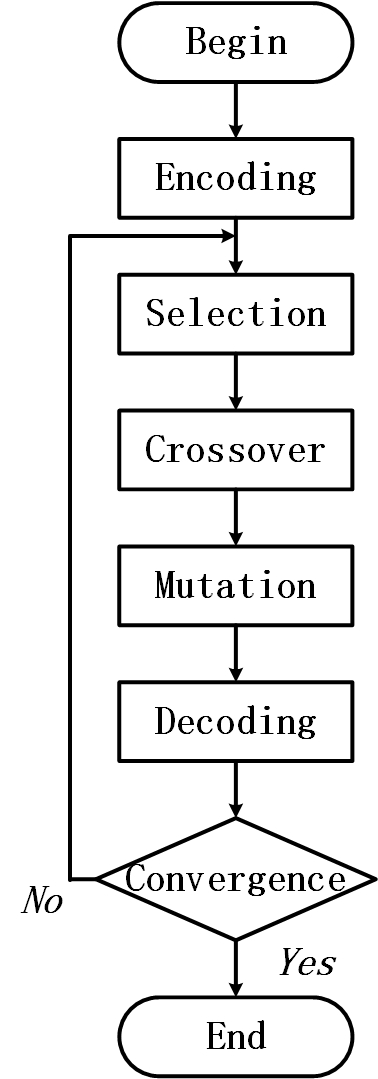
\includegraphics[height=0.6\textheight]{figures/ea_flow.jpg}
  \caption{Evolutionary algorithm}
  \label{fig:evflow}
\end{figure}


Figure \ref{fig:evflow} summarizes the basic process of the evolutionary algorithm. The core 
of the evolutionary algorithm is the design of encoding of candidate 
solutions and the fitness function. The evolutionary algorithm first encodes 
the solutions according to the different requirements of problem. each 
individual in the population represents a solution to the problem. At the 
same time, for each solution of the problem, we also need to design the 
fitness function. The fitness value of different solutions is used to measure 
the adaptability of different individuals. Individuals with high adaptability 
are more likely to survive in the evolution process of population. After 
encoding, there are four steps including initialized population, crossover, 
mutation and selection. The specific operation of initialized population is 
to generate the first generation of population randomly; The cross is to 
product new offspring population by the individual hybridization between 
parents then the mutation is to mutate certain genes in the individuals and 
mutated individuals will be involved in population hybridization to maintain 
the species diversity of the population. As a result, the operation above 
will bring some novel solutions; Finally, the selection is to choose better 
individuals in the whole population according to the natural law of winning. 
In a word, the evolutionary algorithm obtains the optimal solution by the 
evolution of the population.



